\documentclass[12pt,a4paper]{article}

\usepackage[romanian]{babel}
\usepackage{rezstyle}
\usepackage{tikz}
\usetikzlibrary{decorations.markings}

\begin{document}

\begin{titlepage}
    \begin{center}
    {\large \textsc{Universitatea Babes-Bolyai Cluj-Napoca} \par
            \textsc{Facultatea de Matematica si Informatica} \par
            \textsc{Specializarea Matematica} \par }

    \vfill
    
    {\LARGE \textsc{Lucrare de diploma}}
    \null\vskip 1cm
    
    {\huge{Teorema Reziduurilor si aplicatii \par }}           

    \vfill

    \begin{minipage}[b]{0.51\linewidth}
        {\large \emph{Autor :}\\
            Tapalaga Ecaterina Simona}
    \end{minipage}
    \begin{minipage}[b]{0.48\linewidth}
        \begin{flushright}
            {\large \emph{Conducator stiintific:}\\
                Prof. Dr. Salagean Grigore}
        \end{flushright}
     \end{minipage}

    \vfill
    {\large \par Iunie 2013 \par}
    \end{center}
\end{titlepage}

\clearpage

% \tableofcontents

% \clearpage
% Introducere

% \clearpage
% \section{Integrala Riemann-Stieltjes a unei functii complexe de variabila reala}

\begin{definition}
    Fie $f=u+iv$ si $F=U+iV$, iar $[a;b]$ interval din $\R$ . Spunem ca $f$ este integrabila
    Riemann-Stieltjes in raport cu $F$ pe intervalul $[a;b]$ daca $u$ si $v$ sunt integrabile
    Riemann-Stieltjes in raport cu $U$ si $V$ pe $[a;b]$ .

    Notam :
    \begin{equation*}
        \int_a^b f \dd F := \int_a^b u \dd U - \int_a^b v \dd V + i\int_a^b u \dd V + i\int_a^b v \dd U
    \end{equation*}
\end{definition}

\begin{theorem}
    Consideram  $f=u+iv$ ,  $F=U+iV$ , iar $f_n : [a;b] \mapsto \C$ , $F_n : [a;b]\mapsto \C$ ,
     si $\alpha$ , $\beta \in \C$ .

    Au loc urmatoarele proprietati :
    \begin{enumerate}
        \item Daca $f$ este integrabila Riemann-Stieltjes in raport cu $F$ pe $[a;b]$ , atunci $F$ este integrabila
            Riemann-Stieltjes in raport cu $f$ si :
            \[
                \int_a^b f \dd F + \int_a^b F \dd f = f(b) F(b) -f(a)F(a)
            \]
        \item Daca $f$ si $g$ sunt integrabile Riemann-Stieltjes in raport cu $F$ pe $[a;b]$ , atunci
            $\alpha f + \beta g$ e integrabila dupa $F$ si :
            \[
               \int_a^b (\alpha f + \beta g) \dd F = \alpha \int_a^b f \dd F + \beta \int_a^b g \dd F
            \]
        \item Daca $f$ este continua si $F$ este cu variatie marginita pe $[a;b]$ , atunci f este
            integrabila pe $[a;b]$ in raport cu $F$.
        \item Fie $(f_n)_{n \in \mathbb{N}}$ un sir de functii continuue ce converge uniform catre
            $f$ pe $[a;b]$ si $(F_n)_{n \in \mathbb{N}}$ un sir de functii cu variatie marginita
            care converge punctual catre $F$, iar sirul $\mathrm{V}(F_n, [a;b])$ marginit.
            Atunci avem ca:
            \[
                \lim_{\substack{
                        n \to \infty \\
                        k \to \infty
                    }} \int_a^b f_n \dd F_k = \int_a^b f \dd F
            \]
        \item Daca $f$ e continua, $F$ derivabila si $F'$ continua, atunci :
            \[
                \int_a^b f \dd F = \int_a^b f(t) F'(t) \dd t
            \]
        \item Fie $c \in (a;b)$ si $f$ integrabila in raport cu $F$ pe $[a;b]$, atunci $f$
            este integrabila in raport cu $F$ si pe $[a;c]$, si pe $[c;b]$, iar :
            \[
                \int_a^b f \dd F = \int_a^c f \dd F + \int_c^b f \dd F
            \]
        \item Daca $f$ e integrabila in raport cu $F$ pe $[a;b]$, si $h:[a';b'] \mapsto [a;b]$
            $h(a')=a$ si $h(b')=b$, $h$ fiind omeomorfism, atunci $f \circ h$ e integrabila Riemann-Stieltjes pe
            $F \circ H$ si
            \[ \int_a^b f \dd F = \int_{a'}^{b'} (f \circ h) \dd (F \circ H)  \]
    \end{enumerate}
\end{theorem}

\begin{definition}
    Consideram drumul rectificabil $\gamma$, iar $f:\{\gamma\} \mapsto \C$ continua.
    Atunci $f \circ \gamma$ va fi continua pe $[0;1]$ si integrabila in raport cu $\gamma$.
    Aceasta inegrala se numeste integrala complexa a drumului $f$ de-a lungul lui $\gamma$ : 
    \begin{equation*}
        \int_{\gamma} f := \int_{\gamma} f(\zeta) \dd \zeta = \int_0^1 (f \circ \gamma) \dd \gamma
    \end{equation*}
\end{definition}

\begin{theorem}
    Fie $\gamma$ drum rectificabil din $\mathcal{D}(z_0;z_1)$ si $f$ o functie continua din $\{\gamma\}$. Atunci : 
    \begin{enumerate}
        \item Fie $g$ o alta functie continua din $\{\gamma\}$, $\alpha$, $\beta \in \C$ 
            , atunci:
            \[
                \int_{\gamma} \alpha f + \beta g  = \alpha \int_{\gamma} f + \beta \int_{\gamma} g
            \]
        \item 
            \[
                \int_{\gamma^{-}} f = -\int_{\gamma} f
            \]
        \item Fie $\gamma_1$ un alt drum rectificabil din $\mathcal{D}(z_1;z_2)$, atunci :
            \[
                \int_{\gamma \cup \gamma_1} f = \int_{\gamma} f + \int_{\gamma_1} f
            \]
        \item Daca $(\gamma_1, \gamma_2, \cdots, \gamma_n)$ e o descompunere a lui $\gamma$ atunci :
            \[
                \int_{\gamma} f = \sum_{k=1}^{n} \int_{\gamma_k} f
            \]
        \item Daca pentru $\forall t \in [0;1]$ avem ca $|f(\gamma(t))| \leq M$, atunci :
            \[
                \left | \int_{\gamma} f \right | \leq M \cdot \mathrm{V}(\gamma)
            \]
        \item Fie $\gamma$ un drum liniar atunci $\exists z_1, z_2 \in \C$ a.i. :
            \[
                 \int_{\gamma} f = (z_2 -z_1) \int_0^1 f[(1-t)z_1 + tz_2] \dd t
            \]
        \item Fie $f:G\mapsto \C$ continua, G multime deschisa din $\C$ ,
            iar $(\gamma_n)_{n\in\mathbb{N}} \in \mathcal{D}_G$ rectificabile.
            $\{\gamma\} \subset G$ si $(\gamma_n)_{n\in\mathbb{N}}$ converge uniform pe $[0;1]$ catre $\gamma$, iar
            $\mathrm{V}(\gamma_n)$ e multime marginita. Atunci:
            \[
                \lim_{n\to \infty} \int_{\gamma_n} f = \int_{\gamma} f
            \]
        \item Fie $(f_n)_{n\in\mathbb{N}}$ sir de aplicatii continue ,
            $f_n : \{\gamma\} \mapsto \C$ uniform convergent pe $\{\gamma\}$ catre $\C$, atunci
            \[
                \lim_{n\to\infty} \int_{\gamma} f_n = \int_{\gamma} f
            \]
    \end{enumerate}
\end{theorem}

\begin{definition}
    Fie $G\subset \C$ multime deschisa, $f:G\mapsto \C$ si $g \in \mathcal{H}(G)$. Spunem ca $g$
    este primitiva pentru $f$ daca $f = g'$.
\end{definition}

\begin{theorem}[Legatura dintre primitiva si integrala]
    Fie o functie $f:D\mapsto \C$ continua , unde $D$ domeniu din $\C$. Atunci
    \begin{enumerate}
        \item Daca pentru orice contur $\gamma$ din $D$ avem ca $\displaystyle \int_{\gamma} f = 0$, atunci $f$
            admite primitiva pe $D$ .
        \item Daca $g$ este o primitiva a lui $f$ pe $D$, atunci pentru $\forall$ drum rectificabil
            $\gamma$ din $D$ are loc $\displaystyle \int_{\gamma} f = g(\gamma_1) - g(\gamma_0)$. Daca $\gamma$
            e contur (drum rectificabil inchis), atunci avem $\displaystyle \int_{\gamma} f = 0$
    \end{enumerate}
\end{theorem}

\begin{theorem}[Legatura dintre olomorfie si primitiva]
    Fie $D$ un domeniu stelat in $z_0$, iar $d_1, \cdots , d_n$ drepte ce trec prin $z_0$,
    $d$ reuniunea lor. Daca $f:D\mapsto \C$ e continua pe $D$ si derivabila pe $D\setminus d$,
    atunci $f$ admite primitiva pe $D$
\end{theorem}

\begin{theorem}[Cauchy]
    Fie $G$ o multime deschisa. Daca functia $f\in\mathcal{H}(G)$, iar conturul $\gamma$ e omotop cu zero
     in $G$, atunci
     \[
        \int_{\gamma} f = 0
     \]
\end{theorem}


\section{Zerourile functiilor olomorfe}

\begin{definition}
    Fie $G\subset \C$ deschisa, iar $f \in \mathcal{H}(G)$. Daca $\exists$ un punct $z\in G$ a.i.
    $f(z) = 0$, atunci $z$ se numeste zerou al functiei $f$. Daca $\exists$ un $k\in\mathbb{N}^{*}$
    a.i. :
    \[
        f(z) = f'(z) = \cdots = f^{k-1}(z) = 0
    \]
    si $f^{k}(z) \neq 0$, atunci $z$ se numeste zerou multiplu de ordin $k$ pentru $f$

    Pentru $k=1$ il numim pe $z$ zerou simplu.
\end{definition}

\begin{theorem}
    Daca $z$ este un zerou multiplu de ordin $k$ al functiei $f \in \mathcal{H}(G)$ , atunci
    $\exists g \in \mathcal{H}(G)$ a.i.
    \[
        g(x) \neq 0 \text{ si }  f(x) = (x-z)^k g(x) \forall x \in G
    \]
\end{theorem}

\begin{theorem}
    Fie $D \subset \C$ domeniu si $f,g : D\mapsto \C$ functii olomorfe pe $D$. Urmatoarele afirmatii
    sunt echivalente:
    \begin{enumerate}
        \item $f \equiv g$ ;
        \item $\exists$ un punct $a\in D$ a.i. $f^{(k)}(a) = g^{(k)}(a)\; \forall k \in \mathbb{N}$ ;
        \item $ \{z \in D \colon f(z) = g(z)\} \neq \emptyset$ .
    \end{enumerate}
\end{theorem}

\begin{theorem}[Zerourile unei functii olomorfe]
    Fie $D \subset \C$ domeniu si $f\in \mathcal{H}(G)$ nu este identic nula pe $D$, iar $z_0 \in D$
    este un zerou al lui $f$, atunci $\exists r=r(z_0)>0$  a.i. $\mathcal{U}(z_0;r) \subset D $
    si $f(z) \neq 0, z\in \dot{\mathcal{U}}(z_0;r)$ .
\end{theorem}

\begin{theorem}[Maximul modulului]
    Fie $D \subset \C$ domeniu si $f:D\mapsto \C$ o functie olomorfa. Daca $\exists$ un punct
    $z_0 \in D$ a.i. $|f(z)| \leq |f(z_0)|$, $\forall z \in D $, atunci $f$ este constanta.
\end{theorem}

\begin{theorem}[Lema lui Schwarz]
    Fie functia $f$ olomorfa pe $\mathcal{U}(0;1)$ a.i. $f(0) = 0$ si $|f(z)| < M$,
    $z\in \mathcal{U}$, $M>0$. Atunci:
    \[
        |f(z)| \leq M |z| \text{ , } z \in \mathcal{U} \text{ si } |f'(0)| \leq M
    \]

    Daca $\exists z_0 \in \dot{\mathcal{U}}(z_0;r)$ a.i. $|f(z_0)| = M |z_0| $ sau daca
    $|f'(0)| = M$, atunci $\exists \alpha \in \C $ a.i. $|\alpha| = M $ si $f(z) = \alpha z$,
    $z \in \mathcal{U}$
\end{theorem}

\section{Serii Laurent}

\begin{definition}
    Se numeste seria Laurent in jurul lui $z_0 \in \C$ :
    \begin{equation*}
        \sum_{n=-\infty}^{\infty} a_n(z-z_0)^n =
            \cdots + \frac{a_{-n}}{(z-z_0)^n} + \cdots + \frac{a_{-1}}{z-z_0} + a_0 + \cdots a_n(z-z_0)^n + \cdots
    \end{equation*}
    unde $a_n \in \C$ si se numesc coeficientii seriei.

    Daca $\forall n < 0$ avem $a_n = 0$ spunem ca seria Laurent se reduce la o serie de puteri.

    \begin{align*}
        &\sum_{n=1}^{\infty} a_{-n}(z-z_0)^{-n} \text { se numeste partea principala, iar } \\
        &\sum_{n=0}^{\infty} a_n(z-z_0)^n \text { se numeste partea tayloreana}.
    \end{align*}
\end{definition}

\begin{theorem}[Coroanei de convergenta]
    Fie $\displaystyle \sum_{n=-\infty}^{\infty} a_n(z-z_0)^n$ serie Laurent si folosim notatiile :
    \begin{align*}
        r &= \overline{\lim_{n \to \infty}} \sqrt[n]{|a_{-n}|} \\
        \frac{1}{R} &=\overline{\lim_{n \to \infty}} \sqrt[n]{|a_n|}
    \end{align*}
    In conditiile in care $r<R$, avem:
    \begin{enumerate}
        \item $\mathcal{U}(z_0;r;R) = \{z \colon r < |z-z_0| < R\}$
            coroana de convergenta a seriei Laurent converge absolut si uniform pe compacte.
        \item
            \[
                \sum_{n=-\infty}^{\infty} a_n(z-z_0)^n \text{ diverge in }
                    \C \setminus \overline{\mathcal{U}}(z_0;r;R) \text{ .}
            \]
        \item
            \[
                f(z) = \sum_{n=-\infty}^{\infty} a_n(z-z_0)^n \in \mathcal{H}(\mathcal{U}(z_0;r;R)) \text{ .}
            \]
    \end{enumerate}
\end{theorem}

\section{Index unei curbe}

\begin{definition}
    Fie $\gamma$ un drum rectificabil din $\C$ si $z_0 \in \C \setminus \{ \gamma \}$.
    Numim indexul lui $\gamma$ in raport cu $z_0$ :
    \begin{equation*}
        n(\gamma;z_0) := \frac{1}{2 \pi i} \int_{\gamma} \frac{\dd \zeta}{\zeta - z_0}
    \end{equation*}
\end{definition}

\begin{theorem}
    \begin{enumerate}
        \item Fie $\gamma_1$ si $\gamma_2$ drumuri rectificabile din $\C$
            si $z_0 \in \C \setminus \{\gamma_j\}$, $j=\overline{1,2}$. Daca $\gamma_1 \sim \gamma_2$
            in $\C \setminus\{z_0\} \implies n(\gamma_1;z_0) = n(\gamma_2;z_0)$ .
        \item Daca $\gamma_1$ si $\gamma_2$ drumuri rectificabile din $\C$ a.i.
            $\gamma_1(1) = \gamma_2(0)$, $z_0 \notin \{\gamma_j\}$, $j=\overline{1,2}$ atunci
            $n(\gamma_1 \cup \gamma_2; z_0) = n(\gamma_1; z_0) + n(\gamma_2; z_0)$
            \begin{align*}
                \gamma_1 \cup \gamma_2 &: [0;1] \mapsto \C \\
                (\gamma_1 \cup \gamma_2)(t) &=
                    \left \{
                    \begin{aligned}
                        \gamma_1(2t)\;,\; t \in \left [0; \frac{1}{2} \right] \\
                        \gamma_2(2t - 1)\;,\; t \in \left [\frac{1}{2}; 1 \right]
                    \end{aligned}
                    \right .
            \end{align*}
        \item $n(\gamma^{-}; z_0) = - n(\gamma; z_0)$, unde $\gamma$ drum rectificabil pe $\C$
            $z_0 \notin \{\gamma\}$, unde  $\gamma^{-}(t) = \gamma(1-t) $, $t \in [0;1]$ .
    \end{enumerate}
\end{theorem}

\begin{theorem}[Teorema indexului]
    Fie $\gamma$ un contur din $\C$. Atunci
    \begin{equation*}
        n(\gamma;z)\in\Z \text{ , } \forall z \in \C \setminus \{\gamma\} \text{ .}
    \end{equation*}
    
\end{theorem}

\begin{definition}
    Fie $\gamma$ contur din $\C$. $\gamma$ se numeste \emph{contur Jordan} daca
    $\gamma$ contur simplu ($\gamma|_{(0;1)}$ - functie injectiva) si $n(\gamma;z) = 1$,
    $\forall z \in (\gamma)$, unde $(\gamma)$ e domeniul marginit cu frontiera $\gamma$.
\end{definition}

\begin{theorem}[Formulele lui Cauchy pentru contururi]
    Fie $G \subset \C$ deschisa, $f \in \mathcal{H}(G)$, $\gamma$ contur din $G$,
    $\gamma \underset{G}{\sim} 0$. Atunci :
    \begin{equation}
        n(\gamma;z) f^{(k)}(z) = \frac{k!}{2 \pi i} \int_{\gamma} \frac{f(\xi)}{(\xi-z)^{k+1}}
        \;,\; \forall z \in G \setminus \{\gamma\} \;,\; k \in \mathbb{N}
    \end{equation}
\end{theorem}

\section{Functii meromorfe}

\begin{definition}
    Fie $f : \widetilde{G} \mapsto \C$, unde $\widetilde{G}$ multime deschisa din $G$.
    Spunem ca $f$ este meromorfa pe $\widetilde{G}$ si notam $f\in \mathcal{M}(\widetilde{G})$ daca
    $\exists$ o multime $E$ care sa fie alcatuita numai din punctele eliminabile, respectiv poli
    ai functiei $f$ si $f$ sa fie olomorfa pe $\widetilde{G} \setminus E$.
\end{definition}

\begin{definition}
    Fie functia $f \in \mathcal{M}(\widetilde{G})$, unde $\widetilde{G}$ multime deschisa
    din  $\C$, $z_0 \in \widetilde{G}$, $n \in \Z$. Spunem ca $f(z)$ este divizibila cu
    $(z-z_0)^n$ daca $\exists k >0$ si o functie $h$ olomorfa pe $\mathcal{U}(z_0;k)$ a.i.
    $h(z_0) \neq 0$, $\mathcal{U}(z_0;k) \subset \widetilde{G}$ si
    $f(z) = (z-z_0)^n h(z)$, $\forall z \in \dot{\mathcal{U}}(z_0;k)$ .
\end{definition}

\begin{definition}
    Numim \emph{ordinul} lui $f$ in $z_0$:
    \begin{equation}
        o (f;z_0) := \max \{n \in \Z \colon f(z) \text{ divizibila cu } (z-z_0)^n \}
    \end{equation}
\end{definition}

\begin{theorem}[Proprietatii ale ordinului]
    Daca $f_1,\; f_2 \in \mathcal{M}(\widetilde{G}), \; z_0 \in \widetilde{G}$, atunci :
    \begin{enumerate}
        \item $ o (f_1 f_2; z_0) = o(f_1; z_0) + o(f_2; z_0)$ ;
        \item $\displaystyle o \left( \frac{f_1}{f_2} ; z_0\right) = o(f_1;z_0) - o(f_2;z_0)$ ;
        \item Daca $D \subset \widetilde{G}$ si $\displaystyle \sum_{z \in D} o(f;z)$ finita ,
            atunci $\displaystyle o(f;D) := \sum_{z \in D} o(f;z) $  si se numeste ordinul
            functiei $f$ pe $D$ .
    \end{enumerate}

    Daca functia $f \in \mathcal{M}(\widetilde{G})$, $\widetilde{G}$ - multime dechisa din $\C$
    $z_0 \in \widetilde{G}$ , atunci:
    \[
        o(f;z_0) =
            \left \{
            \begin{aligned}
                 n \text{,} && \text{ daca } z_0 \text{ este un zerou de ordin n pentru } f \\
                 0 \text{,} &&\text{ daca } z_0 \text{ punct regular pentru } f \text { dar nu se anuleaza}\\
                -n \text{,} &&\text{ daca } z_0 \text{ pol de ordin n pentru } f
            \end{aligned}
           \right.
    \]
\end{theorem}

\begin{definition}
    $o(f;z) := \infty$, cand $f \equiv 0$, iar $z \in \widetilde{G}$ .
\end{definition}

\begin{theorem}[Teorema lui Cauchy relativa la zerouri si poli]
    Fie $\widetilde{G}$ multime deschisa, $f \in \mathcal{M}(\widetilde{G})$, $f \neq 0$
    $g \in \mathcal{M}(\widetilde{G})$, $\gamma$ contur din $\widetilde{G}$ care nu trece
    prin niciun zerou, respectiv pol al functiei $f$ a.i. $\gamma \underset{G}{\sim} 0$.
    Atunci : 
    \[
        \sum_{z \in \widetilde{G}} n(\gamma;z)\cdot o(f;z) \cdot g(z)  \text{ este finita si}
    \]
    \[
        \int_{\gamma} \frac{f'(z)}{f(z)} g(z) \dd z = 2 \pi i \sum_{z \in G} n(\gamma;z) \cdot o(f;z) \cdot g(z) \text{  .}
    \]
\end{theorem}
% \section{Teorema Reziduurilor}

\begin{theorem}
    Fie functia $f\in \mathcal{H}(G)$, unde $G \subset \C$ multime deschisa.
    Notam cu $\rho$  mutimea tuturor punctelor singulare izolate ale lui $f$
    Fie $\widetilde{G}:=G \cup S $, iar $\gamma$ un contur in $G$ omotop cu zero
     in $\widetilde{G}$
    \begin{align*}
        \text{Atunci suma: }
        &\sum_{z \in \widetilde{G}} {n(\gamma;z) Rez(f;z)}
        \text{ este finita si}  \\
        \int_{\gamma} f(z) \mathrm{d}z = 2\pi i &\sum_{z \in \widetilde{G}} n(\gamma;z) Rez(f;z)
    \end{align*}
    \begin{proof}
        $\exists \varphi:[0;1]^2 \mapsto G$ deformare continuua,
        $k = \varphi ([0;1]^2) \subset \widetilde{G}$ compact.

        Fie
        \begin{align*}
            r &:= \frac{1}{2} \mathrm{d} \left(k, \C \setminus \widetilde{G}\right)
            \\
            D &:= \bigcup_{z\in k} \mathcal{U}(z;r)
        \end{align*}

        $k \subset D \subset \overline{D} \subset \widetilde{G}$

        $\gamma$ omotop cu $0$ in $D$

        $\overline{D} \cap \rho$ finita
                $\implies \exists \{b_1, \dotsc, b_k \} = \overline{D} \cap \rho$

        Fie $\Pi_{k}(z)$ partea principala a dezvoltarii lui $f$ in $b_k$

        Deci, functia $\displaystyle g := f - \sum_{k=1}^{n} \Pi_k$
        olomorfa mai putin in $b_k$ admite o prelungire olomorfa $g_1$ la $D$ .
        \begin{align*}
            \int_{\gamma}  g &= \int_{\gamma} g_1 = 0 \\
                           g &= g_1 |_{D=\{b_1, \dotsc, b_k\}}\\
            \implies \int_{\gamma} f &= \sum_{k=1}^{n} \int_{\gamma} \Pi_k
        \end{align*}

        Calculam
        \[
            \int_{\gamma} \Pi_k \text{ , unde }
            \Pi_k(z) = \sum_{m=1}^{\infty} \frac{a^{(k)} - m }{(z - b_k)^m}
        \]

        Seria este uniform convergenta pe $\forall$ parte compacta din
        $\C \setminus \{b_a \} \implies$ uniform convergenta pe
        $\{ \gamma \} \implies$ putem integra termen cu termen si
        \[
            \int_{\gamma} \frac{\mathrm{d}}{z-b_k} m = 0 , \forall m>1
        \]
        Functia $\displaystyle \frac{1}{(z-b_n)^m}$ admite primitiva si
        $\displaystyle
            \int_{\gamma} \frac{\mathrm{d}z} {z - b_k} = 2 \pi i \cdot n(\gamma;b_n) \cdot a_{-1}^{(k)}
        $ deci
        \[
            \int_{\gamma} f = 2 \pi i \sum_{k=1}{n} n(\gamma; b_k) Rez(f;b_n)
        \]

        Trebuie sa mai aratam ca $\forall z_0 \in \widetilde{G} \setminus(D \cap \rho)
        \colon n(\gamma; z_0)\cdot Rez(f;z_0) = 0$

        Intr-adevar, daca pentru
        $z_0\in \widetilde{G} \setminus (D\cap\rho)$ avem
        $Rez(f;z_0) \neq 0 \implies z_0 \in \rho $, deci $z_0\notin D$ si
        \[
            n(\gamma;z_0) = \frac{1}{2 \pi i} \int_{\gamma}
            \frac{\mathrm{d} \xi}{\xi - z_0} = 0
        \]
        caci $h(\xi) = \frac{1}{\xi - z_0}$ olomorfa pe $D$ si $\gamma$ omotop cu zero
        \[
            \implies \int_{\gamma} f = 2 \pi i \sum_{z\in \widetilde{G}} n(\gamma;z) \cdot Rez(f;z)
        \]

    \end{proof}
\end{theorem}

\section{Puncte singulare izolate}

\begin{definition}
    Fie $G\subset \C$ multime deschisa si $f\in\mathcal{H}(G)$. Punctul $z_0 \in \C$
    se numeste punct singular izolat pentru functia $f$ daca $z_0 \notin G$, dar
    $\exists p>0$ a.i
    $\mathcal{\dot{U}}(z_0;p)\subset G \implies f \in \mathcal{H}(\mathcal{\dot{U}}(z_0;p))$
\end{definition}

\begin{observation}
    De exemplu functiile $\frac{\sin(z)}{z}$ , $\frac{1}{z}$, $e^{\frac{1}{z}}$
    au singularitati izolate in $z=0$
\end{observation}

\begin{observation}
    Daca $z_0$ este un punct singular izolat pentru $f\in\mathcal{H}(G)$, iar
    $p>0$ a.i $\mathcal{\dot{U}}(z_0;p)\subset G$ , atunci $f$ admite o dezvoltare in
    serie Laurent de forma
    \[
        f(z) = \sum_{k=-\infty}^{\infty} a_{k}(z-z_0)^{k},\quad z\in \mathcal{\dot{U}}(z_0;p)
    \]
    Coeficientul $a_{-1}$ al termenului $(z-z_0)^{-1}$ se numeste reziduul functiei $f$
    in $z_0$ si se noteaza cu $a_{-1} = Rez(f;z_0)$
\end{observation}

\begin{definition}
    Fie $G \subset \C$ multime deschisa, $f\in\mathcal{H}(G)$ , iar $z_0$ punct singular
    izolat al functiei $f$. Spunem ca:
    \begin{enumerate}
        \item  $z_0$ este punct eliminabil daca $f$ se extinde olomorf la $\Omega \cup \{z_0\}$
        \item  $z_0$ este pol daca $lim_{z \to z_0} f(z) = \infty$
        \item  $z_0$ este punct esential izolat daca $\nexists$ limita a lui $f$ in $z_0$
        \item Un punct $z$ este regular pentru $f$ daca $z$ este eliminabil pentru $f$
        sau $f$ este derivabila in $z$
    \end{enumerate}
\end{definition}

\section{Calcularea reziduului intr-un pol}
\begin{enumerate}
    \item Daca $z_0$ este un pol de ordin $k$ pentru $f$ atunci
    \[
    Rez(f;z_0) = \frac{1}{(k-1)!}\lim_{z \to z_0} \left[(z-z_0)^k f(z) \right]^{(k-1)}
    \]
    \item In cazul unui punct singular esential reziduul se calculeaza cu ajutoril dezvoltarii
    in serie Laurent
    \item Intr-un punct regular reziduul este 0
\end{enumerate}

\section{Aplicatii ale teoriei reziduurilor la calculul unor integrale definite reale}

% tre sa fie tipul 1
\begin{tip}[1]
    Fie integrala $\displaystyle I=\int_{0}^{2\pi} R(\sin x, \cos x) \mathrm{d} x$, unde
    $R(u,v)$ este o functie rationala reala ce nu are poli pe cercul $u^2+v^2=1$

	\[
        \text{Atunci } \int_{0}^{2\pi} R(\sin x , \cos x) \mathrm{d} x =
        2\pi i \sum_{z\in \mathcal{U}(0;1)} Rez(f;z)
    \]
    \[
        \text{unde } f(z) = \frac{1}{z} R\left(\frac{z-\frac{1}{z}}{2i}, \frac{z+\frac{1}{z}}{2} \right)
    \]

    \begin{proof}
        Utilizand formulele lui Euler:
        \[
            \cos x = \frac{e^{ix}+e^{-ix}}{2}, \sin x = \frac{e^{ix}-e^{-ix}}{2i} x \in \R
        \]
        si substitutia $e^{ix}=z$, avem ca

        \begin{align*}
            \int_{0}^{2\pi} R(\sin x , \cos x) \mathrm{d} x &=
                \int_{\partial \mathcal{U}(0;1)}
                    R\left(\frac{z-\frac{1}{z}}{2i}, \frac{z+\frac{1}{z}}{2} \right)
                \frac{\mathrm{d} z}{iz}            
            \implies 
						\\
						\int_{0}^{2\pi} R(\sin x , \cos x) \mathrm{d} x 
							&= -i \int_{\partial \mathcal{U}(0;1)} f(z) \mathrm{d}z            
            \overset{T.Rez}{\implies}
						\\
						\int_{\partial \mathcal{U}(0;1)} f(z) \mathrm{d}z &=
                2\pi i \sum_{|z|<1} Rez(f;z)            
            \implies 
						\\
						\int_{0}^{2\pi} R(\sin x , \cos x) \mathrm{d} x &=
                2\pi \sum_{|z|<1} Rez(f;z)
        \end{align*}


    \end{proof}
\end{tip}


\begin{tip}
    Fie $R$ o functie rationala reala , $R=P\setminus Q$ unde $P$ si $Q$ polinoame de
    grad $n$ , respectiv $m$, $Q(x)\neq 0 \forall x\in \R$,
    $lim_{z\to\infty} z f(z) =0, (n \leq m-2)$
    Atunci ,
    \[
        \int_{-\infty}^{\infty} R(x) \mathrm{d} x = 2\pi i \sum_{Im z = 0} Rez(f;z)
    \]
    \begin{proof}
        $\exists M,r_1 >0 $ a.i
        \[
            \left|\frac{P(x)}{Q(x)} \right| \leq \frac{M}{|x|^2} , \quad |x| \geq r_1
        \]
    \end{proof}
\end{tip}

% \section{Aplicatii ale teoriei reziduurilor la calculul unor integrale definite reale}

% tre sa fie tipul 1
\begin{tip}[1]
    Fie integrala $\displaystyle I=\int_{0}^{2\pi} R(\sin x, \cos x) \dd x$, unde
    $R(u,v)$ este o functie rationala reala ce nu are poli pe cercul $u^2+v^2=1$

    \[
        \text{Atunci } \int_{0}^{2\pi} R(\sin x , \cos x) \dd x =
        2\pi i \sum_{z\in \mathcal{U}(0;1)} \Rez(f;z)
    \]
    \[
        \text{unde } f(z) = \frac{1}{z} R\left(\frac{z-\frac{1}{z}}{2i},\; \frac{z+\frac{1}{z}}{2} \right)
    \]

    \begin{proof}
        Utilizand formulele lui Euler:
        \[
            \cos x = \frac{e^{ix}+e^{-ix}}{2}\; ,\quad \sin x = \frac{e^{ix}-e^{-ix}}{2i} x \in \R
        \]
        si substitutia $e^{ix}=z$, avem ca

        \begin{align*}
            \int_{0}^{2\pi} R(\sin x , \cos x) \dd x &=
                \int_{\partial \mathcal{U}(0;1)}
                    R\left(\frac{z-\frac{1}{z}}{2i}, \frac{z+\frac{1}{z}}{2} \right)
                \frac{\dd z}{iz}
            \implies
                        \\
                        \int_{0}^{2\pi} R(\sin x , \cos x) \dd x
                            &= -i \int_{\partial \mathcal{U}(0;1)} f(z) \dd z
            \overset{T.Rez}{\implies}
                        \\
                        \int_{\partial \mathcal{U}(0;1)} f(z) \dd z &=
                2\pi i \sum_{|z|<1} \Rez(f;z)
            \implies
                        \\
                        \int_{0}^{2\pi} R(\sin x , \cos x) \dd x &=
                2\pi \sum_{|z|<1} \Rez(f;z)
        \end{align*}


    \end{proof}
\end{tip}


\begin{tip}
    Fie $R$ o functie rationala reala , $R=P / Q$ unde $P$ si $Q$ polinoame de
    grad $n$ , respectiv $m$, $Q(x)\neq 0 \quad \forall x\in \R$,
    $\displaystyle \lim_{z\to\infty} z f(z) =0, (n \leq m-2)$

        Atunci
    \[
        \int_{-\infty}^{\infty} R(x) \dd x = 2\pi i \sum_{\Ima z = 0} \Rez(f;z)
    \]
    \begin{proof}
        $\exists M,r_1 >0 $ a.i
        \[
            \left|\frac{P(x)}{Q(x)} \right| \leq \frac{M}{|x|^2} , \quad |x| \geq r_1
        \]
        \[
            \int_{r_1}^{\infty} \frac{1}{x^2} \dd x \text{ converge } \implies
            \int_{r_1}^{\infty} \frac{P(x)}{Q(x)} \dd x \text{ converge }
        \]
        Analog
        \[
           \int_{ - \infty}^{- r_1} \frac{P(x)}{Q(x)} \dd x \text{ converge }
        \]

                \[
                    \text{Dar } \frac{P}{Q} \text{ continuua pe } [- r_1, r_1] \implies
            \exists \int_{- r_1}^{r_1} \frac{P(x)}{Q(x)} \dd x
                \]

        \[
            \int_{- \infty}^{0} \frac{P(x)}{Q(x)} \dd x \text{ si }
            \int_{0}^{\infty} \frac{P(x)}{Q(x)} \dd x \text{ converg } \implies
            \int_{- \infty}^{\infty} \frac{P(x)}{Q(x)} \dd x \text{ converge }
        \]

        Fie $r>0$ suficient de mare astfel incat toti polii lui $f$ din semiplanul
        superior sa fie continuti in $\Omega_r$, unde $\Omega_r = \{z\in\C \colon |z| < r,\quad \Ima z > 0\}$ .

                Fie $\gamma_r(t) = r e^{\pi i t}, t\in[0;1], \gamma=[-r;r]\cup \gamma_r$.

                Atunci $\gamma = \partial \Omega_r$, iar $(\gamma) = \Omega_r$
        $\overset{T. Rez}{\implies}$

        \begin{equation*}
            \int_{\gamma} f(z) \dd z = 2 \pi i \sum_{z \in \Omega_r} \Rez(f;z)
                = 2 \pi i \sum_{\Ima z >0} \Rez(f;z)  \qquad (*)
        \end{equation*}

        Pe de alta parte
        \begin{equation*}
            \int_{\gamma} f(z) \dd z = \int_{\gamma_r} f(z) \dd z + \int_{-r}^{r} f(x) \dd x \qquad (**)
        \end{equation*}

        Din $(*)$ si $(**)$ trecand la limita $\implies$

        \[
            2 \pi i \sum_{\Ima z >0} \Rez(f;z) = \lim_{r\to \infty} \int_{\gamma_r} f(z) \dd z
                + \int_{- \infty}^{\infty} f(x) \dd x
        \]

        \[
            \text{Dar, } \lim_{z\to\infty} z f(z)=0 \implies \lim_{r\to\infty} \int_{\gamma_r} f(z) \dd z = 0
        \]
        \[
            \implies \int_{- \infty}^{\infty} f(x) \dd x = 2 \pi i \sum_{\Ima z >0} \Rez(f;z)
        \]
    \end{proof}
\end{tip}


\begin{tip}
    Fie $R$ o functie rationala reala de forma
             $\displaystyle R = \frac{P}{Q}$,
             $Q(x) \neq 0$ ,
             $ x \in \R$ ,
             grad $Q >$ grad  $P+1$ si
             $\displaystyle \lim_{|z|\to\infty} R(z) = 0  $

             Atunci
             \[
                    \int_{- \infty}^{\infty} R(x) e^{ix} \dd x \text{ converge si}
                    \int_{- \infty}^{\infty} R(x) e^{ix} \dd x = 2 \pi i \sum_{\Ima z >0} \Rez(f;z)
              \]
            unde $f(z) = R(z) e^{iz}$ .

    \begin{proof}
        Fie $r>0$ suficient de mare a.i. toti polii functiei $f$ din semiplanul superior
        sa fie continuti in $D$, unde $D=\{z\in\C \colon |z| < r ;\ \Ima\ z >0\}$

        Fie $C = \partial D \implies C = [-r;r] \cup \gamma_r$
        \[
            \overset{T.\Rez}{\implies} \int_{C} f(z) \dd z = 2 \pi i \sum_{\Ima\ z >0} \Rez(f;z)
        \]

        \begin{displaymath}
            \left.
                \begin{aligned}
                    \text{Dar } \int_{C} f(z) \dd z
                        = \int_{-r}{r} f(x) \dd x + \int_{\gamma_r} f(z) \dd z \\
                        r \to \infty
                \end{aligned}
            \right \}
            \implies
        \end{displaymath}

        \begin{align*}
            \implies 2\pi i \sum_{\Ima\ z >0 } \Rez(f;z)
                &= \int_{-\infty}{\infty} f(x) dx + \lim_{r\to\infty} \int_{\gamma_r} f(z) \dd z
            \\
                &= \int_{-\infty}^{\infty} \frac{P(x)}{Q(x)} e^{ix} \dd x
                   + \lim_{r\to\infty} \int_{\gamma_r} \frac{P(z)}{Q(z)} e^{iz} \dd z
        \end{align*}

        \[
            g(z) = \frac{P(z)}{Q(z)}
        \]
        deci,
        \[
            \lim_{z\to\infty}g(z) = 0 \overset{L.Jordan}{\implies}
            \lim_{r\to\infty} \int_{\gamma_r} g(z) e^{iz} \dd z = 0
        \]
        Asadar,
        \[
            \int_{-\infty}^{\infty} \frac{P(x)}{Q(x)} e^{ix} \dd x
                =2 \pi i \sum_{\Ima\ z >0} \Rez(f;z)
        \]
    \end{proof}
\end{tip}

\begin{tip}
    Fie integrala
    \[
        I = \int_{-\infty}^{\infty} f(x) e^{i \alpha x}\dd x
    \]
    unde $f=P/Q$ , $Q(x)\neq 0$ , $x \in \R$ , $grad\ P = k$ , $grad\ Q =p$,
    iar $p \geq k+1$ .

    Daca $\alpha > 0$, atunci:
    \[
        I = \int_{-\infty}^{\infty} f(x) e^{i \alpha x}\dd x
            =2 \pi i \sum_{\Ima\ z >0} \Rez(g;z)
    \]
    , unde $g(z) = f(z) e^{i \alpha z}$.

    \begin{proof}
        Observam ca
        $\displaystyle
            \exists \int_{-\infty}^{\infty} f(x) e^{i \alpha x}\dd x
        $
        si este convergenta.
        Intr-adevar, pentru ca $\displaystyle p\geq k+1 \implies \lim_{z\to\infty}f(z) = 0$.
        Dar $\displaystyle f'(z) = \frac{h(z)}{Q^2(z)}$, unde $h$ este un polinom
        de grad cel mult $k+p-1$.

        Fie $x_0$ zeroul lui $h$ de modul maxim $\implies f'(x)$
        are semn constant pentru $x>|x_0| \implies f(x) $ monotona pentru $x>|x_0|$.

        Fie $x_1,\ x_2 \in \R \text{ cu } x_2 > x_1 > |x_0|$
        \[
            \begin{aligned}
            \text{Cum } \lim_{z\to\infty} f(z) = 0 \implies
                &\text{ fie } f>0 \text{ si } \lim_{x\to\infty} f(x) = 0^+ , x >|x_0|\\
                &\text{ fie } f<0 \text{ si } \lim_{x\to\infty} f(x) = 0^- , x >|x_0|
            \end{aligned}
        \]
        Aplicand a doua teorema de medie din calculul integral
        $\implies \exists \xi \in (x_1;x_2)$ a.i.
        \[
            \int_{x_1}^{x_2} f(x) \cos \alpha x\ \dd x
                = f(x_1) \int_{x_1}^{\xi} \cos \alpha t\ \dd t
                + f(x_2) \int_{\xi}^{x_2} \cos \alpha t\ \dd t
        \]
        \[
            \implies \left | \int_{x_1}^{x_2} f(x) \cos \alpha x\ \dd x  \right |
                \leq \frac{2}{\alpha} |f(x_1)| + \frac{2}{\alpha} |f(x_2)|
        \]
        \[
            \text{Stiind ca } \lim_{z\to\infty} f(z) = 0 \implies
                \forall \epsilon > 0 \quad \exists \delta(\epsilon) > 0 \text{ a.i. } |f(x)|<\frac{\epsilon \alpha }{4}
            x > \delta(\epsilon)
        \]
        Deci,
        \[
            \left | \int_{x_1}^{x_2} f(x) \cos \alpha x\ \dd x  \right |
                \leq \frac{2}{\alpha} \big[ |f(x_1)|+ |f(x_2)| \big] < \epsilon ,
        \]
        \[
            x_2 > x_1 > \max\{|x_0|,\ \delta(\epsilon)\}
                \implies \int_{0}^{\infty} f(x)\cos \alpha x\ \dd x
                \text{ converge }
        \]
        Analog $\exists$ si converge
        \[
            \int_{0}^{\infty} f(x)\sin \alpha x \dd x
        \]
        \[
            \implies \int_{0}^{\infty} f(x) e^{i \alpha x} \dd x
        \]
        este deasemenea convergenta.

        Fie $\Omega_r = \{z \in \C \colon |z|<r ; \Ima\; z>0\}$ ce contine toti polii functiei
        $g$ din semiplanul superior
        \[
            \overset{T.Rez}{\implies} \int_{\partial \Omega_r} g(z) \dd z
                = 2 \pi i \sum_{z \in \Omega_r} \Rez(g;z)
                = 2 \pi i \sum_{\Ima\; z > 0} Rez(g;z)
        \]
        Dar
        \[
            \int_{\partial \Omega_r} g(z) \dd z
                = \int_{-r}^{r} f(x)e^{i \alpha x} \dd x
                + \int_{\gamma_r} g(z) \dd z
        \]
        \[
            \overset{L.Jordan}{\implies} \lim_{r \to \infty} \int_{\gamma_r} g(z) \dd z = 0
        \]
        \[
            \overset{r\to\infty}{\implies} \int_{-\infty}^{\infty} f(x)e^{i \alpha x} \dd x
                = 2 \pi i \sum_{\Ima\; z > 0} \Rez(g;z)
        \]
    \end{proof}

\end{tip}
% 
\begin{aplicatie}
    Sa se calculeze integrala :
    \[
        I = \int_{-\infty}^{\infty} \frac{\dd x}{a^4+x^4} \quad , \text{ unde } a > 0.
    \]
    \begin{proof}

    Este o integrala de tipul $\mathrm{II}$
    \begin{align*}
        &\left .
            \begin{aligned}
                P(x) &= 1 \\
                Q(x) &= a^4 +x^4
            \end{aligned}
        \right \}
        grad\; Q > grad\; P+2 \\
        & f(z) = \frac{1}{a^4 +z^4}
    \end{align*}
    \[
        a^4 +z^4 = 0 \implies z^4 = -a^4 = a^4 (\cos \pi + i\sin \pi)
    \]
    \[
        \implies z_k = a \left( \cos \frac{\pi+2k\pi}{4} + i \sin \frac{\pi+2k\pi}{4} \right)
            , k=\overline{0,3}
    \]
    unde $z_k, k=\overline{0,3}$ sunt poli simpli pentru $f$.
    \begin{align*}
        z_0 &= a \left(\frac{\sqrt 2}{2} + i\frac{\sqrt 2}{2} \right)
            = \frac{a}{\sqrt 2} (1+i) \\
        z_1 &= \frac{a}{\sqrt 2} (-1+i) \\
        z_2 &= \frac{a}{\sqrt 2} (-1-i) \\
        z_3 &= \frac{a}{\sqrt 2} (1-i)
    \end{align*}
    \[
        I = 2 \pi i \sum_{\Ima  \; z_k >0} \Rez(f;z_k)
    \]
    \[
        \implies I = 2 \pi i [\Rez(f;z_0) + \Rez(f;z_1)]
    \]
    \[
        \Rez(f;z_k) = \lim_{z \to z_k} (z-z_k) \frac{1}{z^4+a^4}
            \EqConformCaz
            \lim_{z \to z_k} \frac{1}{4z^3}
            = - \frac{z_k}{4a^4}
    \]
    Deci,
    \[
        I = 2 \pi i \left[ \frac{a}{\sqrt 2} (1+i -1 +i) \right]
            = \frac{2 \pi i \cdot a \cdot 2i}{\sqrt 2}
            \implies I = - \frac{4 \pi a}{\sqrt 2}
    \]
    \end{proof}
\end{aplicatie}

\begin{aplicatie}
    Sa se calculeze integrala
    \[
        I = \int_{-\infty}^{\infty} \frac{\cos x}{x^2+a^2} \dd x, \text{ unde } a>0 .
    \]
    \begin{proof}
        Este o integrala de tip $\mathrm{III}$ :
        \begin{align*}
            \text{Fie } I_1 &= \int_{-\infty}^{\infty} \frac{\cos x}{x^2+a^2} \dd x \\
            \text{si }  I_2 &= \int_{-\infty}^{\infty} \frac{\sin x}{x^2+a^2} \dd x (= 0 \text{ pe ca e impara}) \\
            \text{ si fie } I &= I_1 + i I_2 \\
            \implies I &= \int_{-\infty}^{\infty} \frac{e^{ix}}{x^2+a^2} \dd x
        \end{align*}

        \begin{align*}
            &\left .
                \begin{aligned}
                    P(x) &= 1 \\
                    Q(x) &= a^2 +x^2
                \end{aligned}
            \right \}
            \begin{aligned}
                grad\; Q &\geq grad\; P+1 \\
                2 &\geq 1
            \end{aligned}
            \\
            &f(z) = \frac{e^{iz}}{a^2 +z^2}
        \end{align*}

        $a^2 +z^2 = 0 \implies z_{1,2} = \pm i a$ , dar doar $z_1 = i a$
        pol de gradul I $\in$ semiplanul superior
        \[
            \implies I = 2 \pi i\; \Rez(f;z_1) = 2 \pi i\; \Rez(f;i a)
        \]
        \[
            \Rez(f;i a) = \lim_{z \to ia} (z - i a) \frac{e^{iz}}{z^2+a^2}
                = \frac{e^{-a}}{z + i a} = \frac{e^{-a}}{2ia}
        \]
        \[
            \implies I = 2 \pi i \frac{e^{-a}}{2ia} = \frac{e^{-a}\pi}{a}
        \]
        \[
            I_1 = \Rea \; I \quad I_2=\Ima \; I
                \implies I_1 = \frac{e^{-a}\pi}{a}; \quad I_2 = 0
        \]
    \end{proof}
\end{aplicatie}

\begin{theorem}
    Fie $f \in \mathcal{M}(\C)$ si $z_1 , \dotsc , z_k$ poli ai functiei $f$ cu
    reziduurile $u_1, \dotsc , u_k$.
    Daca $f(z) \neq 0$, $z \in \Z$, $z_j \notin \Z$, $j=1, \dotsc, k$,
    iar $f(z) = O(z^{-2}), z\to \infty$, atunci
    \[
        \sum_{-\infty}^{\infty} f(\varphi) = -\pi \sum_{j=1}^{k} \Rez ( \ctg \pi z \cdot f(z);z_j )
    \]
\end{theorem}

\begin{aplicatie}
    Sa se calculeze \[ \sum_{n=1}^{\infty} \frac{1}{n^4 + 1}\]
    \begin{proof}
        Se vede ca
        \[
            \sum_{-\infty}^{\infty} \frac{1}{n^4 + 1} = 1 + 2 \sum_{n=1}^{\infty} \frac{1}{n^4 + 1}
        \]
        Fie $\displaystyle f(z) = \frac{1}{z^4+1}$, atunci $f\in \mathcal{M}(\C)$ , cu polii simpli $\pm 1, \pm i$.
        \[
            \Rez(f;z_k) = \lim_{z \to z_k} \frac{z-z_k}{z^4+1}
                \EqConformCaz \lim_{z \to z_k} \frac{1}{4z^3}
                =\frac{z_k}{-4}
        \]
        \begin{align*}
          \sum_{-\infty}^{\infty} \frac{1}{n^4 + 1}
            &= - \pi \left[-\frac{1}{4} \ctg \pi + \frac{1}{4} \ctg(-\pi)
              - \frac{i}{4} \ctg i\pi + \frac{i}{4}\ctg(-i\pi)\right] \\
            &= \frac{\pi}{4}[\ctg \pi + \ctg \pi + i\ctg i\pi + i\ctg i\pi] \\
            &= \frac{\pi}{2} \ctg \pi + \frac{\pi}{2} \mathrm{cth}\; \pi
        \end{align*}
        \[
            \text{Deci, } 1 + 2 \sum_{n=1}^{\infty} \frac{1}{n^4 + 1}
                = \frac{\pi}{2} \ctg \pi + \frac{\pi}{2} \mathrm{cth}\; \pi
        \]
        \[
            \implies \sum_{n=1}^{\infty} \frac{1}{n^4 + 1}
                = \frac{\pi}{4} [\ctg \pi + \mathrm{cth}\; \pi ] - \frac{1}{2}
        \]

    \end{proof}
\end{aplicatie}

\subsection{Calcularea unei integrale pe un arc de curba simplu si rectificabil, dar nu inchis}

    In acest caz putem incerca sa formam o curba inchisa $\gamma_0 \cup \gamma_1$
    a.i. sa poata sa se aplice teorema reziduurilor , iar integrala pe noua curba
    $\gamma=\gamma_0 \cup \gamma_1$ sa se poata calcula cu
    reziduuri direct sau sa aiba o relatie simpla cu integrala cautata.

    Daca integrala este improprie , fiind limita unei alte integrale
    \[
        \int_{\gamma_0}= \lim_{\gamma \to \gamma_0} \int_{\gamma}
    \]
    atunci si arcul adaugat va varia si vom putea calcula integrala improprie
    cunoscand limita $\int_{\gamma_1}$ si daca  suma reziduurilor din domeniu $G$
    variabil are limita cunoscuta:
    \[
        \int_{\gamma_0} f \dd z = - \lim \int_{\gamma_1} f \dd z + 2 \pi i \lim \sum \Rez (f;z)
    \]

    \begin{aplicatie}
        Sa se calculeze
        \[
            I = \int_{0}^{\infty} \frac{\cos ax}{\ch \pi x} \dd x , a \in \R
        \]
        \begin{proof}
            \[
                f(z) = \frac{\cos az}{\ch \pi z}
            \]
            Polii acestei functii sunt simpli , $z = (2k+1)\frac{i}{2}$, $k \in \Z$
            Pentru a evita seria de reziduuri care este divergenta alegem conturul

            \begin{center}
                \begin{tikzpicture}[decoration={markings,
                    mark=at position 1cm with {\arrow[line width=1pt]{>}},
                    mark=at position 3cm with {\arrow[line width=1pt]{>}},
                    mark=at position 5cm with {\arrow[line width=1pt]{>}},
                    mark=at position 7cm with {\arrow[line width=1pt]{>}},
                    mark=at position 9cm with {\arrow[line width=1pt]{>}},
                    mark=at position 11cm with {\arrow[line width=1pt]{>}},
                    }]

                    \draw[help lines,->] (-3,0) -- (3,0) coordinate (xaxis);
                    \draw[help lines,->] (0,-1) -- (0,3) coordinate (yaxis);

                    \path[draw,line width=0.8pt,postaction=decorate] (-2,0) node[below] {$-R$} -- (2,0) node[below] {$R$} -- (2,2) -- (-2,2) -- cycle;

                    \node[below] at (xaxis) {$Re$};
                    \node[left] at (yaxis) {$Im$};
                    \node[below left] {$O$};
                    \node[below left] at (0,2) {$i$};
                \end{tikzpicture}
            \end{center}

            Pe latura $z=R + i y \quad ( 0 \leq y \leq 1)$

            \begin{align*}
              \left| i \int_{0}^{1} \frac{\cos a (R+iy)}{\ch \pi (R+iy)} \dd y \right|
                 &= \left| \int_{0}^{1} \frac{e^{ia(R+iy)} + e^{-ia(R+iy)}}
                                           {e^{\pi(R+iy)} + e^{-\pi(R+iy)}} \dd y \right|
              \\ &< \frac{\int_{0}^{1} (e^{-ay} + e^{ay}) \dd y}{e^{\pi R} - e^{-\pi R}}
                \to 0
            \end{align*}
            \[
                \text{Ramane : } 2 \int_{0}^{R} \frac{\cos ax}{\ch \pi x} \dd x
                    + \int_{0}^{R} \left[
                                    - \frac{\cos a(i+x)}{\ch \pi (i+x)}
                                    - \frac{\cos a(i-x)}{\ch \pi (i-x)}
                                   \right] \dd x
                \longrightarrow 2 \pi i \Rez \left(f;\frac{i}{2}\right)
            \]
            Stiind ca :
            \begin{align*}
                \ch \pi( x \pm i) &= -\ch \pi x
                \\
                \cos a(x \pm i) &= \cos ax \cdot \ch a \mp \sin ax \cdot \sh a
            \end{align*}
            obtinem ca :
            \[
                2(1+\ch a) \int_{0}^{R} \frac{\cos ax}{\ch \pi x} \dd x
                    \longrightarrow 2 \pi i \Rez \left(f;\frac{i}{2}\right)
            \]
            \[
                \Rez \left(f;\frac{i}{2} \right)
                    = \lim_{z\to\frac{i}{2}} \left( z- \frac{i}{2}\right) \frac{\cos az}{\ch \pi z}
                    = \frac{\cos \frac{ai}{2}}{\pi \sh \frac{\pi i}{2}}
                    = \frac{\ch \frac{a}{2}}{\pi i \sh \frac{\pi}{2}}
                    = \frac{\ch \frac{a}{2}}{\pi i}
            \]
            \[
                \implies I = 2 \pi i \frac{\ch \frac{a}{2}}{\pi i} = 2 \ch \frac{a}{2}
            \]
        \end{proof}

    \end{aplicatie}

    \subsection{Aplicatii la dezvoltari in serie}

    \begin{theorem}
        Fie $f(z)$ o functie meromorfa ai carei poli formeaza un sir infinit $z_k \to \infty$
        si $D_n$ un domeniu marginit de o curba rectificabila $\gamma_n$ si care nu trece
        prin nici un pol $z_k$.
        \[
            \text{Atunci : } \int_{\gamma_n} f(z) \dd z = 2\pi i \sum_{k=1}^{n} \Rez (f;z_k) .
        \]
    \end{theorem}

    \begin{observation}\leavevmode
        \begin{enumerate}
            \item Daca $n \to \infty, \gamma_n$ variaza a.i. $D_n$ tinde catre un domeniu
                ce cuprinde toti polii $a_n$. Daca integrala din membrul $\mathrm{I}$ are o limita finita,
                atunci obtinem suma seriei de reziduuri $\displaystyle \sum_{k=1}^{\infty}\Rez(f;z_k)$ insumata
                dupa domeniul $D_n$.
            \item Daca indicele $k$ ia valorile $1,2,\cdots $ si $|z_k|$ sunt strict crescatoare
                $|z_1|<|z_2|< \cdots$ , a.i. intre 2 curbe consecutive sa se afle un singur pol,
                vom obtine suma seriei convergente $\displaystyle \sum_{k=1}^{\infty}\Rez(f;z_k)$ .
            \item Daca  $|z_k|$ si  $|z_{-k}|$ sunt crescatori vom putea obtine suma seriei
                convergente  $\displaystyle \Rez(f;z_0) + \sum_{k=1}^{n}[\Rez(f;z_k)+ \Rez(f;z_{-k})]$ adica :
                \[
                    \sum_{-\infty}^{\infty} \Rez(f;z_k)
                        = \frac{1}{2 \pi i} \lim_{k\to \infty} \int_{\gamma_k} f(z) \dd z
                \]
            \item Fie $f(z)$ o functie mereomorfa avand polii de gradul $\mathrm{I}$ , $z_k \to \infty$ si
                $g(z)$ o functie uniforma cu un numar finit de puncte singulare $a_h$, diferite de
                $z_k$ . Fie $\gamma_n$ cu $n>n_0$ ce contine punctele $a_h$ in interiorul sau.
                Atunci pentru functia $f(z)\cdot g(z)$ avem ca
                \[
                    \Rez(f\cdot g;z_k)=g(z_k) \Rez(f;z_k)
                \]
                Formula din Obs 3 se transforma astfel
                \[
                    \sum_{-\infty}^{\infty} \Rez(f;z_k) g(z_k)
                        = \frac{1}{2 \pi i} \lim_{k\to \infty} \int_{\gamma_k} f(z)g(z) \dd z
                        - \sum_{k\in\C} \Rez(f\cdot g; a_h)
                \]
                A doua suma este nula pentru $g(z)$ functie intreaga
        \end{enumerate}
    \end{observation}

    \begin{aplicatie}
        Sa se calculeza integrala
        \[
            I = \int_{0}^{2 \pi} \frac{\dd x}{a + \cos x}, a>1
        \]
        \begin{proof}
            Se observa ca $I$ este o integrala de tipul $\mathrm{I}$.
            Din formulele lui Euler stim ca:
            \[
                \cos z = \frac{e^{ix}+e^{-ix}}{2}
                , \quad e^{ix} = z \implies \dd x = \frac{\dd z}{iz}
                        \implies \cos x = \frac{z+\frac{1}{z}}{2}
            \]
            \[
                f(z) = \frac{1}{z} \frac{1}{a + \frac{z + 1/z}{2}}
                \implies f(z) = \frac{1}{z^2 + 2az + 1}
            \]
            \[
                I = \int_{\partial\mathcal{U}(0;1)} \frac{\frac{\dd z}{iz}}{a + \frac{z + 1/z}{2}}
                  = - 2i \int_{\partial\mathcal{U}(0;1)} \frac{\dd z}{z^2 + 2az + 1}
            \]
            \[
                z^2 + 2az + 1 = 0 \implies \Delta = 4 a^2 - 4
            \]
            \[
                \implies \left \{
                \begin{aligned}
                    z_1 &= \frac{-2a + \sqrt{4a^2-4}}{2} = -a + \sqrt{a^2 - 1}  \\
                    z_2 &= \frac{-2a - \sqrt{4a^2-4}}{2} = -a - \sqrt{a^2 - 1}
                \end{aligned}
                \right .
            \]

            \begin{align*}
                |z_1| < 1 &\iff |-a + \sqrt{a^2 - 1 }| = a - \sqrt{a^2 -1} < 1 \\
                          &\iff a-1 < \sqrt{a^2 -1} \; \Big{|}^2 \iff a^2 - 2a + 1 < a^2 -1 \\
                          &\iff 2a > 0 \text { Adevarat. }     \\
                |z_2| < 1 &\iff |-a - \sqrt{a^2 - 1 }| < 1 \text{ Fals .}
                \implies z_2 \notin \mathcal{U}(0;1)
            \end{align*}

            Deci, $I = 2 \pi \Rez(f;z_1)$ cu $z_1$ pol simplu :
            \begin{align*}
               \Rez(f;z_1)
                    &= \lim_{z\to z_1}(z-z_1)\frac{1}{z^2+2az+1}
                        \EqConformCaz
                        \lim_{z\to z_1}\frac{1}{2z+2a} \\
                    &= \frac{1}{2(a+\sqrt{a^2 - 1}) + 2a} = - \frac{1}{2\sqrt{a^2-1}}
            \end{align*}
            Asadar ,
            \[
                I = 2 \pi \frac{1}{2\sqrt{a^2 -1}} = \frac{\pi}{\sqrt{a^2-1}}
            \]
        \end{proof}
    \end{aplicatie}

    \begin{theorem}
        Fie functia reala rationala $f=P / Q$, neavand poli pe $[0;1]$, fie $0<\alpha<1$ si
        $\displaystyle \lim_{z\to \infty} f(z) = 0$ .
        Atunci avem ca :
        \[
            \int_{0}^{\infty} \frac{f(x)}{x^\alpha} \dd x
                = \frac{\pi e^{\alpha \pi i}}{\sin \alpha \pi} \sum_{z\in \C^*} \Rez(h;z) ,
        \]
        \[
            \text{unde } h(z) = \frac{f(z)}{z^\alpha} \text{ , iar } z^\alpha = e^{\alpha \log z} ,
        \]
        cu $\log z$ ramura uniforma a aplicatiei multivoce Logaritm.
        \begin{proof}
            Fie $\Gamma $ conturul din imagine:

            \begin{center}
                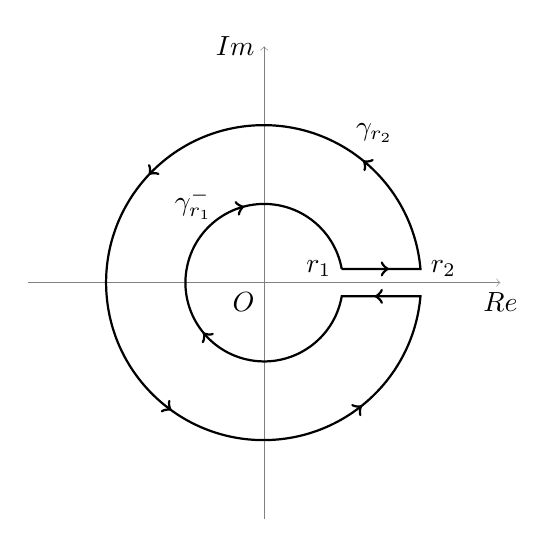
\begin{tikzpicture}[decoration={markings,
                    mark=at position 0.6cm with {\arrow[line width=1pt]{>}},
                    mark=at position 2.6cm with {\arrow[line width=1pt]{>}},
                    mark=at position 5.6cm with {\arrow[line width=1pt]{>}},
                    mark=at position 9cm with {\arrow[line width=1pt]{>}},
                    mark=at position 11.6cm with {\arrow[line width=1pt]{>}},
                    mark=at position 13.8cm with {\arrow[line width=1pt]{>}},
                    mark=at position 16.5cm with {\arrow[line width=1pt]{>}},
                    mark=at position 18.5cm with {\arrow[line width=1pt]{>}},
                    }]

                    \draw[help lines,->] (-3,0) -- (3,0) coordinate (xaxis);
                    \draw[help lines,->] (0,-3) -- (0,3) coordinate (yaxis);

                    \path[draw,line width=0.8pt,postaction=decorate] (10:1) node[left] {$r_1$} -- +(1,0) node[right] {$r_2$} arc (5:355:2) -- +(-1,0) arc (-10:-350:1);

                    \node[below] at (xaxis) {$Re$};
                    \node[left] at (yaxis) {$Im$};
                    \node[below left] {$O$};
                    \node at (-0.9,1) {$\gamma_{r_1}^{-}$};
                    \node at (1.4,1.9) {$\gamma_{r_2}$};

                \end{tikzpicture}
            \end{center}

            Atunci :
            \[
                \int_{\Gamma} g(z) \dd z = 2\pi i \sum_{z\in \C^*} \Rez(g;z)
            \]
            si :
            \[
              \int_{\Gamma} g(z) \dd z
                    = \int_{r_1}^{r_2} \frac{f(x)}{x^\alpha} \dd x
                    + \int_{\gamma_{r_2} } \frac{f(z)}{z^\alpha} \dd z
                    - \int_{r_1}^{r_2} \frac{f(x)}{e^{\alpha[\ln x + 2\pi i]}} \dd x
                    - \int_{\gamma_{r_1}} \frac{f(z)}{z^\alpha} \dd z
            \]

            Deci :
            \[
               (*) \quad 2 \pi i  \sum_{z\in \C^*} \Rez(g;z)
                    = \int_{\gamma_{r_2}} \frac{f(z)}{z^\alpha} \dd z
                    - \int_{\gamma_{r_1}} \frac{f(z)}{z^\alpha} \dd z
                    + (1-e^{-2\pi i \alpha}) \int_{r_1}^{r_2} \frac{f(x)}{x^\alpha} \dd x
            \]

            Cum $\displaystyle \lim_{z\to\infty} f(z) = 0$ urmeaza ca $p \leq k+1$, unde $k$ si $p$
            sunt gradele polinoamelor $P$ respectiv $Q$. Deoarece $\alpha \in (0;1)$, obtinem imediat
            ca :
            \[
                \lim_{z\to\infty} z g(z) = \lim_{z\to\infty} z^{1-\alpha} \frac{P(z)}{Q(z)} = 0
                \text{ si }
                \lim_{z\to 0} z g(z) = \lim_{z\to 0} z^{1-\alpha} \frac{P(z)}{Q(z)} = 0 .
            \]
            Trecand la limita in $(*)$ pentru $r_1 \to 0$ si $r_2 \to \infty$ deducem concluzia teoremei.
        \end{proof}
    \end{theorem}

    \begin{aplicatie}
        Sa se calculeze integrala :
        \[
            I = \int_{0}^{\infty} \frac{\dd x}{\sqrt[3]{x}(x^5+a^5)} , a > 0.
        \]
        \begin{proof}
            Aceasta integrala este de tip $\mathrm{V}$.
            \begin{align*}
                f(x) &= \frac{1}{x^5+a^5} \\
                h(z) &= \frac{1}{z^{1/3}(z^5+a^5)}
            \end{align*}
            \[
                z^5+a^5 = 0 \implies z^5 = -a^5
            \]
            \[
                z_k = a\left( \cos \frac{\pi+2k\pi}{5} + i \sin \frac{\pi+2k\pi}{5} \right)
                , k = \overline{0,4}
            \]
            unde $z_k$ sunt poli simpli.
            \[
                I = \frac {\pi e^{\frac{\pi i}{3}}}{\sin \frac{\pi}{3}}
                    \sum_{k=0}^{4} \Rez(h;z_k)
            \]
            \begin{align*}
                \Rez(h;z_k) &= \lim_{z\to z_k}(z-z_k)\frac{1}{z^{1/3}(z^5+a^5)}
                    \EqConformCaz
                    \frac{1}{z_k^{1/3}} \lim_{z\to z_k} \frac{1}{5z^4}
                    = \frac{1}{z_k^{1/3}} \lim_{z\to z_k} \frac{z}{5z^4}
                    \\
                    &= \frac{1}{z_k^{1/3}} \frac{z_k}{5a^5}
                    = - \frac{z_k^{2/3}}{5a^5}
                    = - \frac{1}{5a^5} e^{\frac{2}{3}\log z_k}
                    = - \frac{1}{5a^5} e^{\frac{2}{3} [\ln a + i \theta(z)]}
                    \\
                    &= - \frac{1}{5a^5} e^{\frac{2}{3} \left[\ln a + i \frac{\pi+2k\pi}{5}\right]}
                    = - \frac{a^{2/3}}{5a^5} e^{\frac{2}{3} \frac{i \pi + 2k\pi}{5}}
                    \\
                I &= -\frac{\pi e^{\frac{\pi i}{3}}}{\frac{\sqrt{3}}{2}} \frac{a^{2/3}}{5a^5}
                    e^{i\frac{2}{3}}
                    \left[e^{\frac{\pi}{5}} + e^{\frac{3 \pi}{5}}
                    + e^{\frac{5 \pi}{5}} +e^{\frac{7 \pi}{5}} +e^{\frac{9 \pi}{5}}
                    \right]
            \end{align*}
        \end{proof}
    \end{aplicatie}
% \section{Aplicatii in teoria functiilor}

Urmatorul rezultat face legatura intre numarul de zerouri si numarul de poli ai unei functii analitice.

\begin{theorem}
    Fie $D \in \C$ domeniu stelat si $f \in \mathcal{M}(D)$ cu zerouurile :
    $a_1, \cdots , a_n \in D$, si polii $b_1, \cdots, b_m \in D$ .
    Atunci pentru orice contur $\gamma$ din $D$ ce evita toate zerourile
    si toti polii lui $f$ avem:
    \[
        \frac{1}{2\pi i} \int_{\gamma} \frac{f'}{f}(\zeta) \dd \zeta
        = \sum_{k=1}^{n} o(f; a_k)\; n(\gamma;a_k)
        + \sum_{l=1}^{m} o(f; b_l)\; n(\gamma;b_l)
    \]
\end{theorem}

O aplicatie a teoremei anterioare e teorema:

\begin{theorem}[Hurwitz]
    Fie $f_1, f_2, \cdots : D \mapsto \C$ un sir de functii ce converge local uniform
    la functia analitica $f : D \mapsto \C$. Daca $\forall i f_i $ nu e identic nula pe D
    atunci $f$ fie e identic nula ori nu are nici un zerou in $D$
\end{theorem}

\begin{theorem}
    Fie $D \in \C$ domeniu stelat si $f \in \mathcal{M}(D)$ cu zerouurile :
    $a_1, \cdots , a_n \in D$, si polii $b_1, \cdots, b_m \in D$.
    Notam:
    \begin{align*}
        N(0) &:= \sum_{k=1}^{n} o(f;a_k) && \text{numarul tuturor zerourilor lui } f \text{ ;} \\
        N(\infty) &:= - \sum_{l=1}^{m} o(f;b_l) && \text{numarul tuturor polilor lui } f \text{ ;}
    \end{align*}
    numarand multiplicitatile.  Fie $\gamma$ din $D$ ce inconjoara cu index 1 toate
    zerourile si toti polii. Atunci avem:
    \[
        \frac{1}{2\pi i} \int_{\gamma} \frac{f'}{f} (zeta) \dd \zeta = N(0) - N(\infty) .
    \]
\end{theorem}

Daca $f$ nu are poli obtinem o formula pentru numarul de zerouri intr-un domeniu.

\begin{aplicatie}[Teorema fundamentala a algebrei]
    Orice polinom $P(z)$ de grad $n$ cu coeficienti complecsi, are exact n radacini complexe.
    \begin{proof}
        Deoarece $\lim_{|z| \to \infty} P(z) = \infty$ , $\exists R > 0$ a.i. $P$ nu are radacini
        $z$ cu $|z| \geq R$ . Numarul de zerouri a lui $P$ e :
        \[
            N(0) = \frac{1}{2\pi i}\int_{|\zeta| = R} \frac{P'(\zeta)}{P(\zeta)} \dd \zeta .
        \]
        Functia $P'/P$ are in $\infty$ un zerou simplu. Seria Laurent in $\infty$ e de forma :
        \[
            \frac{n}{z} + \frac{c_2}{z^2} + \frac{c_3}{z^3} + \cdots (n = grad(P)) .
        \]
        Deci:
        \[
            N(0) = n = grad(P).
        \]
    \end{proof}
\end{aplicatie}

\begin{theorem}[Rouche]
    Fie $f$, $g : D \mapsto \C$ analitice si $\gamma$ un contur din $D$ ce inconjoara
    orice punct din interiorul sau exact o data.
    Daca $|g(\zeta)| < |f(\zeta)| \forall \zeta \in \{\gamma\}$ atunci
    $f$, $f+g$ nu au zerouri in $\{\gamma\}$ si au in interiorul lui $\gamma$ acelasi numar de zerouri
    considerand multiplicitatile.
\end{theorem}

\begin{aplicatie}
    Sa se determine numarul solutiilor ecuatiei $z^4 -8z + 10 = 0 $ in $\mathcal{U}(0;1;3)$
    \begin{proof}
        IMAGINE
        \[
            \mathcal{U}(0;1;3) = \mathcal{U}(0;3)\setminus
                \big(\mathcal{U}(0;1) \cup \partial \mathcal{U}(0;1)\big)
        \]
        \begin{align*}
            N_1 :&= \text{ numarul solutiilor ecuatiei in } \mathcal{U}(0;3) \\
            N_2 :&= \text{ numarul solutiilor ecuatiei in } \mathcal{U}(0;1) \\
            N :&= \text{ numarul solutiilor ecuatiei in } \mathcal{U}(0;1;3)  \\
            N &= N_1 - N_2
        \end{align*}

        Determinam $N_1$. Avem $|z| < 3$.

        Alegem $f(z) = z^4$ si $g(z) = -8z + 10$.
        \begin{align*}
            |z^4| &= 3^4 = 81 \\
            |-8z + 10| &\leq 8|z| + 10 = 24 + 10 = 34 < 81 \implies \\
            |g(z)| &< |f(z)| \text{ pentru } |z| = 2 \overset{T.Rouche}{\implies} \\
            f(z) = 0 \text{ si } & f(z) + g(z) = 0 \text{ au acelasi numar de solutii in }
                \mathcal{U}(0;3) \\
            \implies & N_1 = 4
        \end{align*}

        Determinam $N_2$.
        \begin{align*}
            N'_2 :&= \text{ numarul solutiilor ecuatiei in } \mathcal{U}(0;1) \\
            N''_2 :&= \text{ numarul solutiilor ecuatiei pe } \partial \mathcal{U}(0;1) \\
            N_2 &= N'_2 + N''_2
        \end{align*}
        \begin{align*}
            |z| & = 1 \\
            f(z) & = -8z + 10 \implies g(z) = z^4 \\
            |f(z)| &\leq -8|z| + 10 =  18 \\
            |g(z)| &= |z^4| = 1 < 18 \overset{T.Rouche}{\implies}\\
            f(z) &= 0 \text{ si } f(z) + g(z) = 0 \text{ au acelasi numar de solutii }\\
            -8z + 10 &= 0 \implies z = 2 > 1 \implies N_2 = 0 \text{ numar de solutii in } \mathcal{U}(0;1)\\
            |f(z) + g(z)| &\geq |f(z)| + |g(z)| > 0, |z| = 1 \implies N''_2 = 0
        \end{align*}
        Deci $N = 4-0 = 4$
    \end{proof}
\end{aplicatie}

\begin{aplicatie}
    Fie $P_n(z) = a_0 + a_1 z + \cdots + a_n z^n$, $z \in \C$, unde $a_n \neq 0$ .
    \[
        \text{Fie } \alpha_n = \frac{ \sum_{k=0}^{n-1} |a_k|}{|a_n|}
             \text{ , si } \quad r > \max\{\alpha_n,1\} .
    \]
    Sa se arate ca toate solitiile polinomului $P_n \in \mathcal{U}(0;r)$.
    \begin{proof}
        Fie :
        \begin{align*}
            f(z) &:= a_n z^n \\
            g(z) &:= a_0 + a_1 z + \cdots + a_{n-1}z^{n-1} = P_n(z) - f(z)
        \end{align*}
        Avem :
        \begin{align*}
            |z| &= r \\
            |f(z)| &= a_n |r|^n = |a_n| r^n\\
            |g(z)| &= |a_0 + a_1 z + \cdots + a_{n-1}z^{n-1}| \\
                   &\leq |a_0| + |a_1| |z| + \cdots + |a_{n-1}| |z|^{n-1}\\
                   &= |a_0| + |a_1| r + \cdots + |a_{n-1}|r^{n-1}\\
            \text{Deoarece } & r^k \leq r^{n-1} \forall k = \overline{0,n-1} \\
            |g(z)| &\leq r^{n-1} (|a_0| + |a_1| + \cdots + |a_{n-1}|)
                = r^{n-1}\sum_{k=0}^{n-1}|a_k| \implies \\
            |g(z)| &\leq r^{n-1} \alpha_n |a_n|
                = \frac{\alpha_n r^n |a_n|}{r} = \frac{\alpha_n}{r} |f(z)| \\
            \text{Cum } & \frac{\alpha_n}{r} < 1 \text{ avem ca : }\\
            |g(z)| & < |f(z)| \;,\quad |z| = r
                \overset{T.Rouche}{\implies}\\
            f(z) = 0 & \text{ si } f(z) + g(z) = 0
                \text{ au acelasi numar de solutii in } \mathcal{U}(0;r)
        \end{align*}
        \[
            \left \{
                \begin{aligned}
                    f(z) &= 0 \\
                    P_n(z) &= 0
                \end{aligned}
            \right.
            \text{ au acelasi numar de solutii } \implies N = n
        \]

    \end{proof}
\end{aplicatie}

% \begin{tikzpicture}
% % The axes
% \draw[help lines,->] (-3,0) -- (3,0) coordinate (xaxis);
% \draw[help lines,->] (0,-1) -- (0,3) coordinate (yaxis);

% % The path
% \path[draw,line width=0.8pt] (1,0) node[below] {$\varepsilon$} -- (2,0) node[below] {$r$} arc (0:180:2) -- (-1,0) arc (180:0:1);

% % The labels
% \node[below] at (xaxis) {$x$};
% \node[left] at (yaxis) {$y$};
% \node[below left] {$O$};
% \node at (0.5,1.2) {$C_{\varepsilon}$};
% \node at (1.5,1.8) {$C_{r}$};
% \end{tikzpicture}

% \clearpage

% \nocite{*}
% \bibliographystyle{plain}
% \bibliography{biblio}
\end{document}

